\subsection{TET Histograms and Distance}
	A methods that can be used to find similarity between the TETs is to transform the TETs into histograms and compare these\cite{JAEGER201330}. 
	\begin{figure}[H]
		\centering
		\begin{adjustbox}{width=0.5\textwidth}
			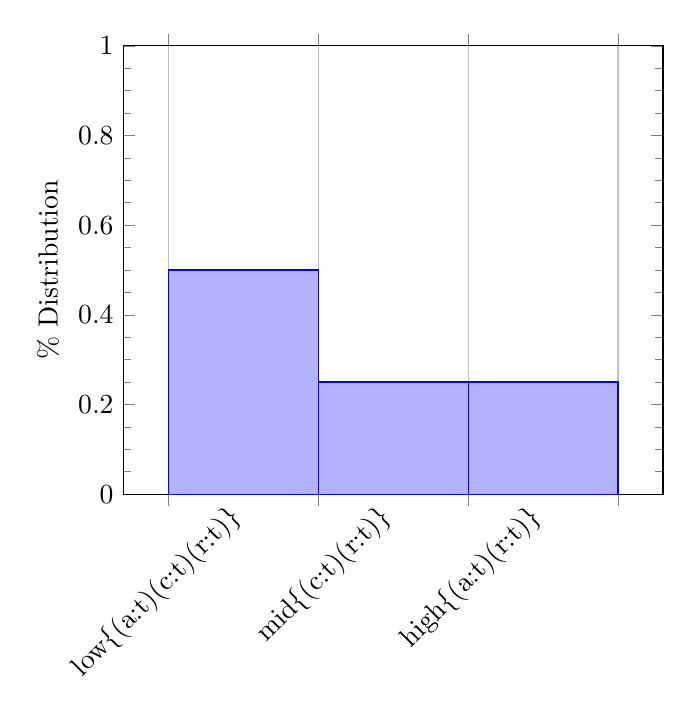
\begin{tikzpicture}
	\begin{axis}[
	ybar interval, 
	ymax=1,ymin=0, 
	minor y tick num = 3,
	ylabel = {\% Distribution},
	symbolic x coords={low\{(a:t)(c:t)(r:t)\}, mid\{(c:t)(r:t)\}, high\{(a:t)(r:t)\}, high\{(y:t)(r:t)\}},
	x tick label style={font=\normalsize, rotate=45, anchor=east},
	]
	\addplot coordinates {(low\{(a:t)(c:t)(r:t)\}, 0.5) (mid\{(c:t)(r:t)\}, 0.25) (high\{(a:t)(r:t)\}, 0.25) (high\{(y:t)(r:t)\}, 0.10)};
	\end{axis}
\end{tikzpicture}

%\begin{tikzpicture}

%\definecolor{bblue}{HTML}{4F81BD}

%\begin{axis}[
%major x tick style = transparent,
%ymin=0,
%bar width=1cm,
%minor y tick num = 3,
%ymajorgrids = true,
%ylabel = {\% distribution},
%symbolic x coords={low\{(a:t)(c:t)(r:t)\}, mid\{(c:t)(r:t)\}, high\{(a:t)(r:t)\}},
%xtick = data,
%x tick label style={font=\normalsize, rotate=45, anchor=east},
%]
%\addplot[ybar , style={bblue,fill=bblue,mark=none}]
%coordinates {(low\{(a:t)(c:t)(r:t)\}, 0.5) (mid\{(c:t)(r:t)\}, 0.25) (high\{(a:t)(r:t)\}, 0.25)};

%\end{axis}
%\end{tikzpicture}
		\end{adjustbox}
		\caption{The TET histogram derived from \autoref{fig:Tet_example}}
		\label{fig:Tethistogram}
	\end{figure}
	
	By using comparing the key for each level in the tree, you can find the structural difference, for example if comparing two TET we know that if the users in the TETs are the same $User(u) == User(u')$ then we work on the same tree and the distance is $0$. The next level is the rating level for \autoref{fig:Tetekempel} this levels histogram would be represented as \autoref{fig:Tethistogram}, on this level we compare low, medium and high by assigning them a numeric value.
	
	On the genre level of the TET structure we find the difference between we see in \autoref{fig:Tethistogram} that $low\{(a:t)(c:t)(r:t)\}$ at this level we have $(a:t)(c:t)(r:t)$ we can use manhatten distance at this level by considering it as a vector there comparison with another histogram with less true genre features than the other at this level can the be compared as seen in \autoref{Eq:manhattencomparason}\cite{singh2013k}.
	
	When comparing two histograms, one histogram might have some elements that the other does not have. For any missing element in a histogram we add the value $0$, and we are thereby able to calculate distance for the missing element.
	
	\begin{equation}\label{Eq:manhattencomparason}
	D(\begin{bmatrix}
	x_{1.1} \\
	x_{1.2} \\
	x_{1.3}
	\end{bmatrix},
	\begin{bmatrix}
	x_{2.1} \\
	x_{2.2}
	\end{bmatrix})= |x_{1.1} - x_{2.1}| + |x_{1.2} - x_{2.2}| + |x_{1.3} - 0|
	\end{equation}
	
	The general formula for these comparisons can be seen in \autoref{eq:compare_tet} and \autoref{Eq:manhattencomparason}
	\begin{equation}\label{eq:compare_tet}
	\begin{split}
	D(h,h') = \sum_{i=1}^{max(|h|,|h'|)} & (D(h^{\downarrow}, h'^{\downarrow})+ D(h_key, h'_key))  \\
	& * distribution(h) * distribution (h')
	\end{split}
	\end{equation}
	
	In \autoref{eq:compare_tet} $h^{\downarrow}$ meaning the TETs next level histogram representation. The $distribution()$ adds the impotence of each of the type of subTETs.
